\chapter{Regularisation and Overfitting}
% Authors: Liangzhi Li (editor), Lekha Iyengar, Subhadarshi Panda, 04/02/19.

\section{Definitions of regularisation}
% Authors: Liangzhi Li (editor), Lekha Iyengar, Subhadarshi Panda, 04/02/19.
\begin{itemize}
    \item[(1)] Regularisation adds prior knowledge to a model i.e. a prior distribution is specified for the parameters
    \item[(2)] Restriction of the set of possible learnable functions
    \item[(3)] "Regularization is any modification we make to a learning algorithm that is intended to reduce its generalization error but not its training error" -- Ian Goodfellow (\cite{Goodfellow-et-al-2016})
\end{itemize}

Definition (3) is commonly used in the context of machine learning (and deep learning).
Intuitions for regularisation and overfitting can be seen in Figure \ref{fig:reg_n_overfitting}.

\begin{figure}
    \centering
    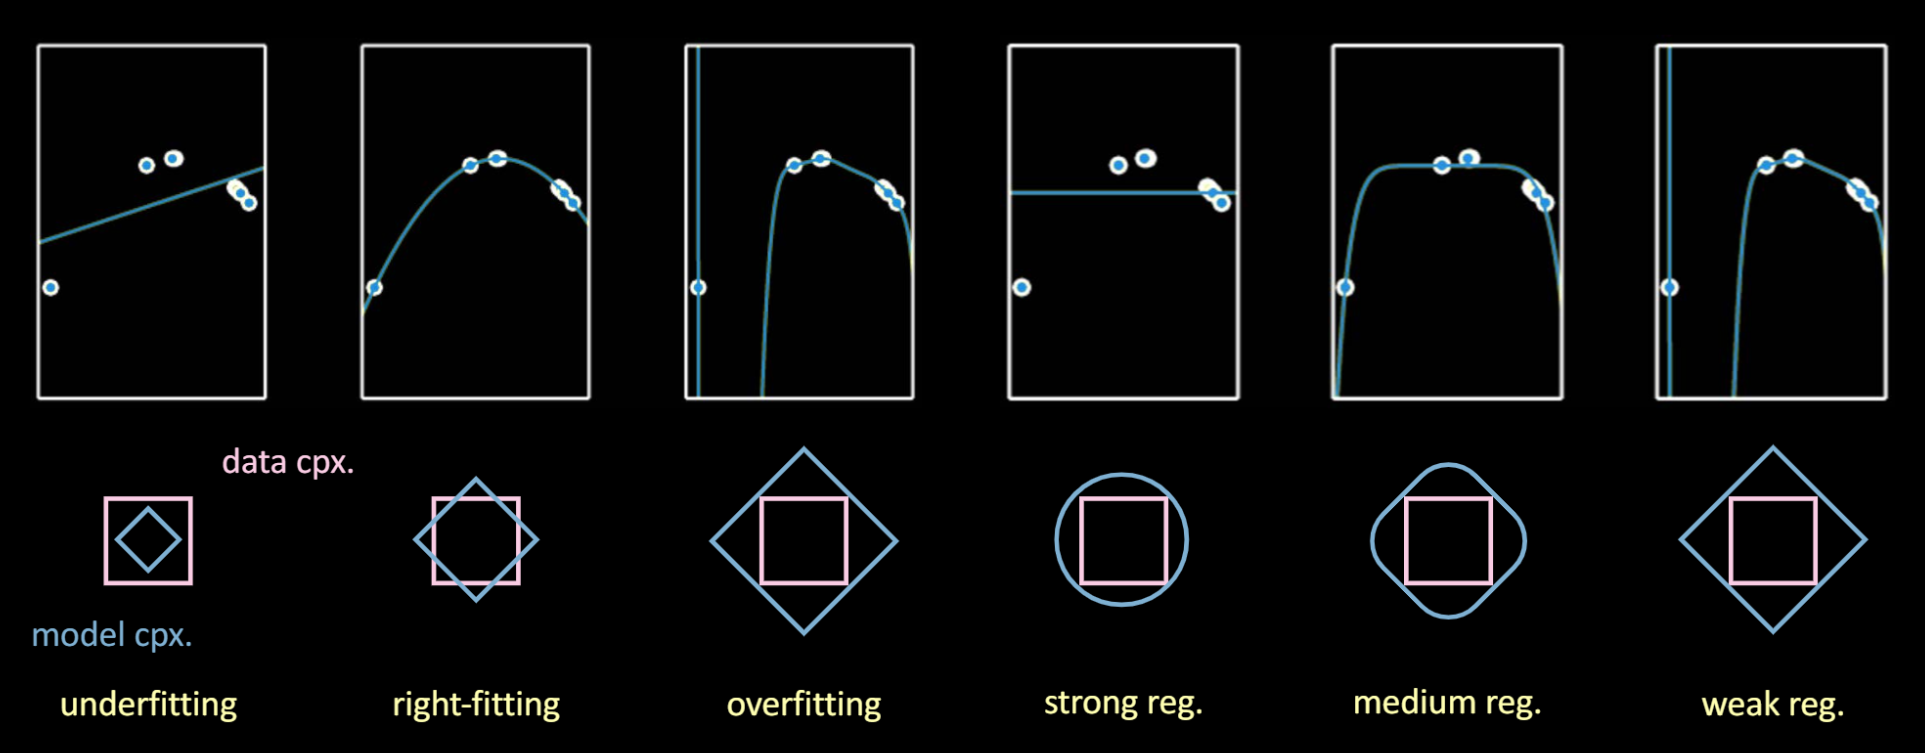
\includegraphics[scale=0.5]{labs/09/images/regularisation_and_overfitting.PNG}
    \caption{Regularisation and overfitting}
    \label{fig:reg_n_overfitting}
\end{figure}

\section{Techniques}
% Authors: Liangzhi Li (editor), Lekha Iyengar, Subhadarshi Panda, 04/02/19.
The following are the regularisation techniques used in neural networks. 
These techniques also reduce overfitting.
    \subsection{Xavier initialization} Random initialization of weights of a neural network before start of training can potentially lead to issues of vanishing gradients or exploding gradients. 
    This in turn can cause the network to learn specific patterns instead of generalizing. This can be avoided using Xavier initialization.
    
    In Xavier initialization, the weights of the network are initialized based on some distribution. 
    The distribution used is typically Gaussian (as in Figure \ref{fig:normal_distribution}) or uniform.
    The original paper \cite{glorot2010understanding} suggested to initialize the weights $W$ of a layer from a distribution with zero mean and variance given by
    
    \begin{align}
        Var(W) = \frac{2}{n_{in} + n_{out}}
    \end{align}
    
    where $n_{in}$ and $n_{out}$ are the number of inputs and outputs of the layer respectively.
    
    \begin{figure}
        \centering
        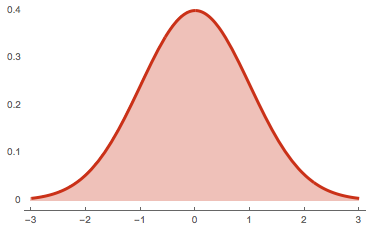
\includegraphics[scale=0.5]{labs/09/images/normal_distribution.png}
        \caption{Normal distribution with zero mean}
        \label{fig:normal_distribution}
    \end{figure}
    
    In PyTorch, Xavier initialization can be done using:
    \begin{itemize}
        \item[(a)] Gaussian or normal distribution: \texttt{torch.nn.init.xavier\_normal\_(tensor, gain=1)}
        \item[(b)] Uniform distribution: \texttt{torch.nn.init.xavier\_uniform\_(tensor, gain=1)}
    \end{itemize}
    
    \subsection{L2 Regularization}
    L2 regularisation can be implemented by penalizing the squared magnitude of all parameters directly in the objective function.
    That is, for every weight $w$ in the network, we add the term $\frac{1}{2}\lambda w^2$ to the objective function, where $\lambda$ is the regularization strength.
    A factor of $\frac{1}{2}$ is used because then the gradient of this term with respect to the parameter $w$ is simply $\lambda w$ instead of $2\lambda w$.
    The L2 regularization has the intuitive interpretation of heavily penalizing peaky weight vectors and preferring diffuse weight vectors. 
    This encourages the network to use all of its inputs a little rather than some of its inputs a lot.
    Lastly, during gradient descent parameter update, using the L2 regularization means that every weight is decayed linearly towards zero, as shown in Figure \ref{fig:L2}.
    
    \begin{figure}
        \centering
        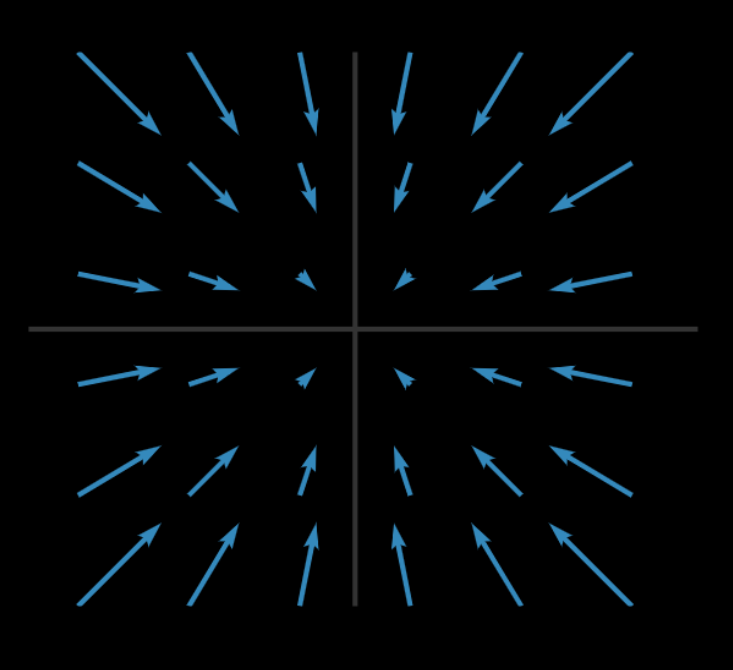
\includegraphics[scale=0.5]{labs/09/images/L2}
        \caption{Gradient descent parameter update using L2 regularisation}
        \label{fig:L2}
    \end{figure}
    
    Alternate names for L2 regularisation are:
    \begin{itemize}
        \item[(a)] Weight decay 
        \item[(b)] Ridge
        \item[(c)] Gaussian prior
    \end{itemize}
    
    In PyTorch, L2 regularisation can be applied using the \texttt{torch.optim} module.
    
    \subsection{L1 Regularization}
    In L1 regularisation, for each weight $w$ in the network we add the term $\lambda |w|$ to the objective function.
    Neurons with L1 regularization end up using only a sparse subset of their most important inputs and become nearly invariant to the noisy inputs.
    Figure \ref{fig:L1} shows the intuition for the gradient descent parameter update using the L1 regularization. The blue unit vectors are L1 vectors and the grey vectors are the corresponding L2 vectors.
    
    \begin{figure}
        \centering
        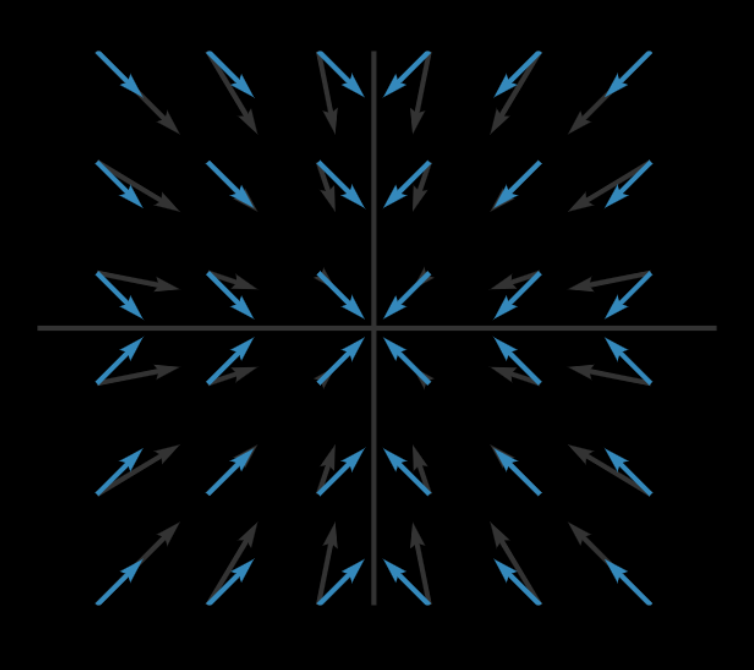
\includegraphics[scale=0.5]{labs/09/images/L1}
        \caption{Gradient descent parameter update using L1 regularisation}
        \label{fig:L1}
    \end{figure}
        
    Alternate names for L1 regularisation are:
    \begin{itemize}
        \item[(a)] LASSO (Least Absolute Shrinkage Selector Operator)
        \item[(b)] Laplacian prior
        \item[(c)] Sparsity prior
    \end{itemize}
        
    In PyTorch, L1 regularisation can be applied using the \texttt{torch.optim} module.
    
    \subsection{Dropout}: Dropout is a regularization technique which is used to prevent overfitting. The technique involves temporarily dropping nodes (hidden and input) along with all its incoming and outgoing connections. During training, dropout removes a unit from the network with probability p(Figure \ref{fig:dropout}). For the input nodes, however, the optimal probability of retention is usually closer to 1. At test time, the node is always present and the weights are multiplied by p.
    This is important because the neurons must have the same output as they had during training time (in expectation).
    $p$ can be considered to be a hyperparameter.

    During training, dropout can be interpreted as sampling a neural network within the full neural network and only updating the parameters of the sampled network based on the input data.
    However, the exponential number of possible sampled networks are not independent because they share the parameters.
    During testing there is no dropout applied, with the interpretation of evaluating an averaged prediction across the exponentially-sized ensemble of all sub-networks.
    
    \begin{figure}
        \centering
        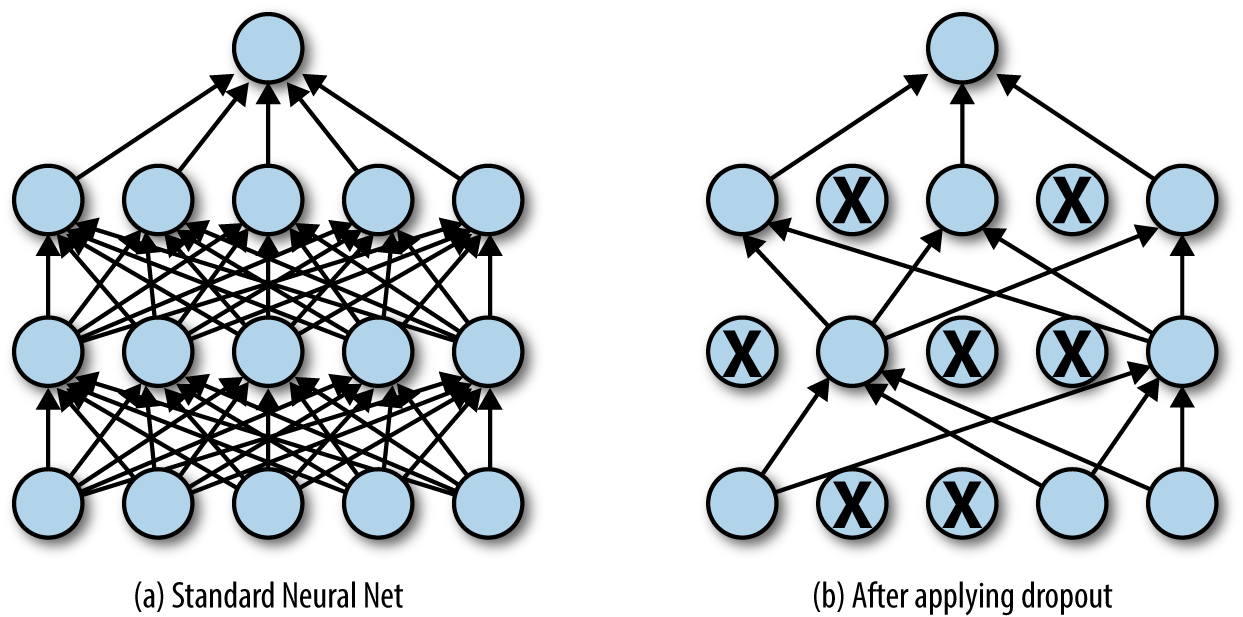
\includegraphics[scale=0.65]{labs/09/images/dropout.png}
        \caption{Dropout Regularization}
        \label{fig:Dropout Regularization}
    \end{figure}
        
    In PyTorch, dropout can be applied using \texttt{torch.nn.Dropout(rate=0.5)}.
    
    Several variants are dropout are also available such as:
    \begin{itemize}
        \item[(a)] \texttt{torch.nn.Dropout2d(rate=0.5)}
        \item[(b)] \texttt{torch.nn.Dropout3d(rate=0.5)}
        \item[(c)] \texttt{torch.nn.AlphaDropout(rate=0.5)}
    \end{itemize}
    
    \subsection{Early stopping} :  
    \begin{figure}
        \centering
        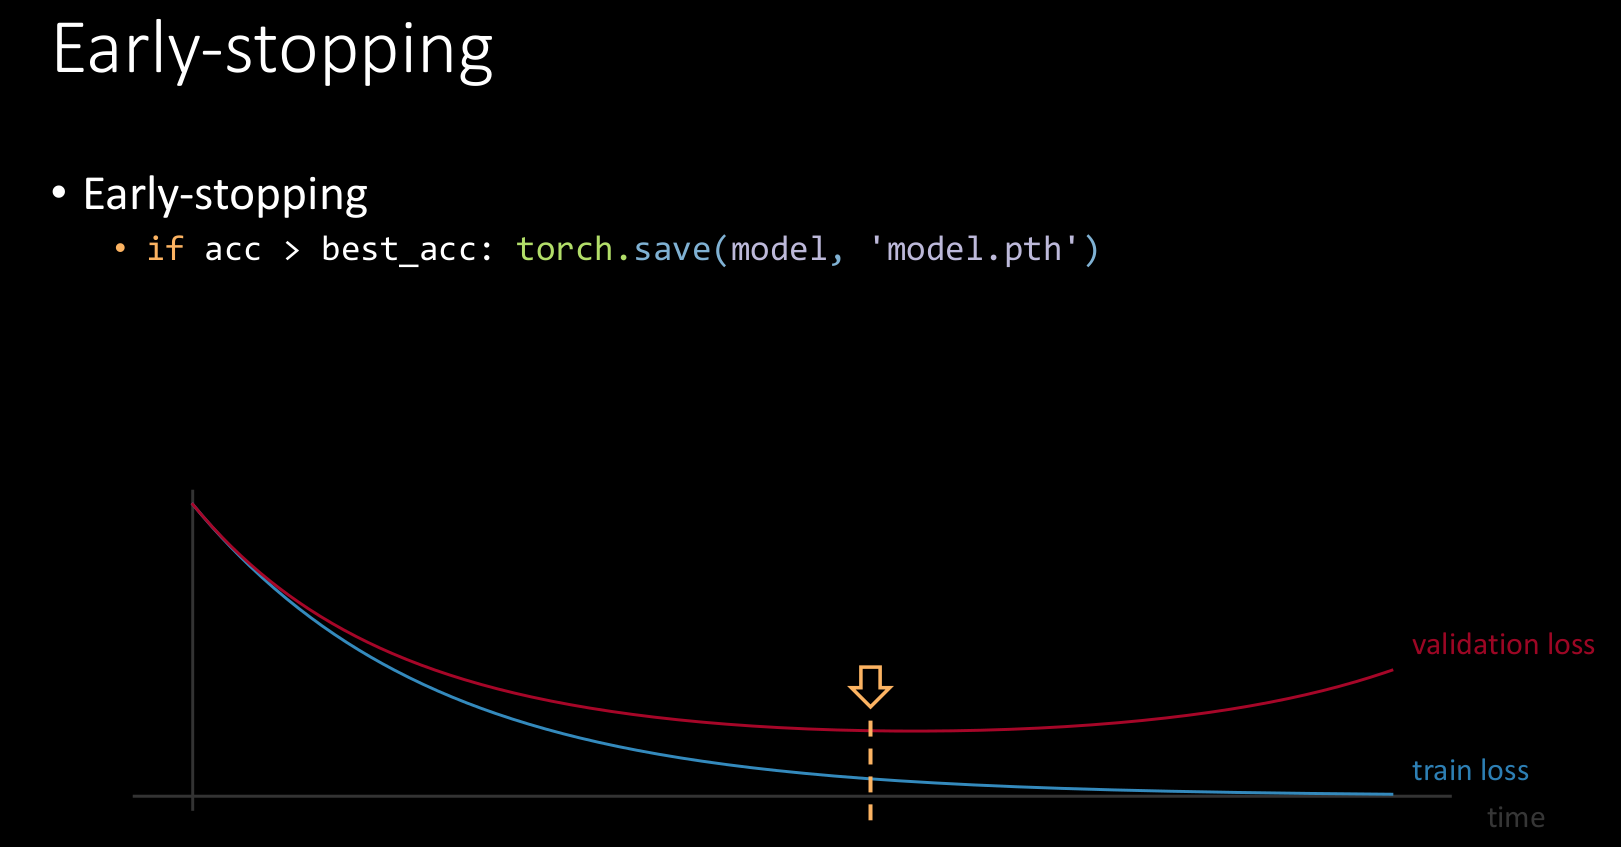
\includegraphics[scale=0.23]{labs/09/images/Early_Stopping.png}
        \caption{Early Stopping}
        \label{fig:Early Stopping}
    \end{figure}
    "All standard neural network architectures such as the fully connected multi-layer perceptron are prone to
    overfitting: While the network seems to get better and better, i.e., the error on the training set decreases, at some point during training it actually begins to get worse again, i.e., the error on unseen examples increases."\cite{early_stopping} 
    If we are using an iterative training algorithm such as gradient descent, we can use early stopping for fighting overfitting.
    The training loss and validation loss decrease with number of epochs in a neural network. 
    However, at a certain point, the validation loss begins to increase while the training loss decreases (See Figure \ref{fig:Early Stopping}).
    We need to stop training at this point as the network starts overfitting here. 
    In each epoch, we check if the validation loss is decreasing; if it is, we save the updated model parameters. 
    At the point where it starts increasing we stop training.

    \subsection{Batch normalization} : Batch normalization reduces the dependence of gradients on the scale of the parameters or on their initial values (reduces internal covariate shift) by fixing the means and variances of layer inputs.
    It also allows each layer to learn independently of other layers. 
    In addition to this, it also acts as a regularizer which helps reduce overfitting.
    This is explained by the authors as - 
    "When training with Batch Normalization, a training example is seen in conjunction with other examples in the mini-batch, and the training network no longer producing deterministic values for a given training example. 
    In our experiments, we found this effect to be advantageous to the generalization of the network." (\cite{DBLP:journals/corr/IoffeS15})
    
    Pytorch provides the following normalization layers :
    \begin{itemize}
        \item[(a)] \texttt{torch.nn.BatchNorm1d(num\_features)}
        \item[(b)] \texttt{torch.nn.BatchNorm2d(num\_features)}
        \item[(c)] \texttt{torch.nn.BatchNorm3d(num\_features)}
    \end{itemize}
    \subsection{Data augmentation} : Another way to fight overfitting is to increase the size of dataset by generating synthetic data. 
    We do this by augmenting the images in dataset using techniques like changing the brightness, cropping, rotating, flipping, scaling and shifting. 
    This helps increase the amount of relevant data and also helps the network generalize better. 
    Adding these synthetically generated images to our training data makes the network robust and invariant to changes. This technique is quite effective in tasks like object detection and speech recognition.
    
    Pytorch has the following transformation functions for data augmentation:
    \begin{itemize}
        \item \texttt{torchvision.transforms.CenterCrop(size)}
        \item \texttt{torchvision.transforms.FiveCrop(size)}
        \item \texttt{torchvision.transforms.ColorJitter(brightness, contrast, saturation, hue)}
        \item \texttt{torchvision.transforms.Grayscale(num\_output\_channels=1)}
        \item \texttt{torchvision.transforms.RandomVerticalFlip(p=0.5)}
        \item \texttt{torchvision.transforms.RandomAffine(degrees, translate, scale, shear)}
        \item \texttt{torchvision.transforms.RandomCrop(size, padding, pad\_if\_needed, fill)}
        \item \texttt{torchvision.transforms.RandomGrayscale(p=0.1)}
        \item \texttt{torchvision.transforms.RandomHorizontalFlip(p=0.5)}
        \item \texttt{torchvision.transforms.RandomRotation(degrees)}
    \end{itemize}

    \subsection{Transfer learning (TL) and Fine Tuning (FT)}:
    "Transfer learning and domain adaptation refer to the situation where what has been learned in one setting (i.e., distribution P 1 ) is exploited to improve generalization in another setting (say distribution P2)." (\cite{Goodfellow-et-al-2016})
    Without transfer learning we would not be able to train networks for tasks with very few examples. 
    We use a model pre-trained on some other related task(Task 1) and use it's knowledge of Task 1 to improve generalization on Task 2. 
    This is done by using the neural network with trained weights and replacing the top layers and retraining these layers. 
    The number of layer replaced depends on the amount of data we have for our task. 
    The type of transfer learning used depends on size of new dataset and its similarity to the original dataset.
    \begin{itemize}
        \item Few data similar to train : If the new dataset is small then we don't fine tune the model as it would lead to overfitting. 
        Since the data is similar to training data, we don't change layers which detect higher level features. 
        We just change the top layer (classifier) and retrain.
        \item Lots data similar to train: We can fine-tune the entire network since we have a lot of data.
        \item Few data different from training data : Since the new dataset is different from the training data, the layers which detect higher level features cannot be reused. These layers may contain dataset specific features. Since our dataset is small, we do transfer learning (retrain the classifier) but we start early. The classifier is trained using activation from an earlier layer.
        \item Lots data different from training data: Since we have a lot of data, we can just train the network and not use transfer learning. 
        We just use the pretrained weights to initialize the network and then train the entire network.
    \end{itemize}
    While doing fine tuning we can use diversified learning rates where we train the classifier on top but the other layers don't change much.